%%%%%%%%%%%%%%%%%%%%%%%%%%%%%%%%%%%%%%%%%%%%%%%%%%%%%%%%%%%%
%%  TEMPLATE IEEE PARA ENTREGA DE INFORMES DE LABORATORIO %% 
%%%%%%%%%  DE LA UNIVERSIDAD MILITAR NUEVA GRANADA  %%%%%%%%
%%%%%%%%%%%  PROGRAMA DE INGENIERÍA MECATRÓNICA  %%%%%%%%%%%
%%%%%%%%%%%%%%%%%%    BOGOTÁ, COLOMBIA    %%%%%%%%%%%%%%%%%%
    %%%%%%%%%%%%%%%%%%%%%%%%%%%%%%%%%%%%%%%%%%%%%%%%%%
    %%%%   AUTOR: SERGIO ANDRÉS CHAPARRO MORENO   %%%%
    %%%%%%%%%%%%%%%%%%%%%%%%%%%%%%%%%%%%%%%%%%%%%%%%%%
    %%%%%%%%%%%%  VERSIÓN 1.0-JULIO 2018  %%%%%%%%%%%%
    %%%%%%%%%%%%%%%%%%%%%%%%%%%%%%%%%%%%%%%%%%%%%%%%%%
\documentclass[journal]{IEEEtran}
\IEEEoverridecommandlockouts
%%%%%%%%%%%%%%%%%%%%%%%%%%%%%%%%%%%%%%
%%%%%%%% PRINCIPALES PAQUETES %%%%%%%%
%%%%%%%%%%%%%%%%%%%%%%%%%%%%%%%%%%%%%%
\usepackage{fancyhdr}
\usepackage{graphicx}
\usepackage[spanish, es-tabla]{babel}
\usepackage[utf8]{inputenc}
\usepackage{color}
\usepackage{hyperref}
\usepackage{wrapfig}
\usepackage{array}
\usepackage{multirow}
\usepackage{adjustbox}
\usepackage{nccmath}
\usepackage{subfigure}
\usepackage{amsfonts,latexsym} % para tener disponibilidad de diversos simbolos
\usepackage{enumerate}
\usepackage{booktabs}
\usepackage{float}
\usepackage{threeparttable}
\usepackage{array,colortbl}
\usepackage{ifpdf}
\usepackage{rotating}
\usepackage{cite}
\usepackage{stfloats}
\usepackage{url}
\usepackage{listings}
\usepackage{amsmath}
\usepackage{makecell}%To keep spacing of text in tables
\setcellgapes{2pt}%parameter for the spacing in tables
%%%%%%%%%%%%%%%%%%%%%%%%%%%%%%%%%%%%%%%%%%%
%%% CREAR Y REESCRIBIR ALGUNOS COMANDOS %%%
%%%%%%%%%%%%%%%%%%%%%%%%%%%%%%%%%%%%%%%%%%%
\newcolumntype{P}[1]{>{\centering\arraybackslash}p{#1}}  %% Se crea un nuevo tipo de columna llamada P.
\newcommand{\tabitem}{~~\llap{\textbullet}~~}
\newcommand{\ctt}{\centering\scriptsize\textbf} %%\ctt abrevia el comando \centering\scriptsize\textbf
\newcommand{\dtt}{\scriptsize\textbf} %%\dtt abrevia el comando \scriptsize\textbf
\renewcommand\IEEEkeywordsname{Palabras clave}
%%%%%%%%%%%%%%%%%%%%%%%%%%%%%%%%%%%%%%%%%%%


% correct bad hyphenation here
\hyphenation{op-tical net-works semi-conduc-tor} %% Con este comando se especifican como pueden seprarse las sílabas adecuadamente en caso una palabra quede en dos lineas diferentes de texto

\graphicspath{ {figs/} }  %%Ruta donde se encuentran las imágenes, que esté vacio indica que las imagenes están dentro de la misma carpeta que contiene el archivo .tex


%%%%%%%%%%%%%%%%%%%%%%%%%%%%%%%%%%%%%%%%%%%%%%%%%%%%%%%%%%
%%%%%%%%%%% ENCABEZADO DE LAS PÁGINAS TIPO UMNG %%%%%%%%%%
%%%%%%%%%%%%%%%%%%%%%%%%%%%%%%%%%%%%%%%%%%%%%%%%%%%%%%%%%%
\newcommand{\MYhead}{\smash{\scriptsize
\hfil\parbox[t][\height][t]{\textwidth}{\centering
\begin{picture}(0,0) \put(-0,-17){\includegraphics[width=10mm]{Universidad Católica Boliviana _San Pablo_ UCB.jpg}} \end{picture} \hspace{6.4cm}
INFORME DE PROYECTO \hspace{5.15cm} Versión 1.0\\
\hspace{6.45cm} INGENIERÍA MECATRÓNICA \hspace{4.65cm} Semestre 2020-1\\
\underline{\hspace{ \textwidth}}}\hfil\hbox{}}}
\makeatletter
% normal pages
\def\ps@headings{%
\def\@oddhead{\MYhead}%
\def\@evenhead{\MYhead}}%
% title page
\def\ps@IEEEtitlepagestyle{%
\def\@oddhead{\MYhead}%
\def\@evenhead{\MYhead}}%
\makeatother
% make changes take effect
\pagestyle{headings}
% adjust as needed
\addtolength{\footskip}{0\baselineskip}
\addtolength{\textheight}{-1\baselineskip}
%%%%%%%%%%%%%%%%%%%%%%%%%%%%%%%%%%%%%%%%%%%%%%%%%%%%%%%%%%
%%%%%%%%%%%%%%%%%%%%%%%%%%%%%%%%
%%%%% INICIO DEL DOCUMENTO %%%%%
%%%%%%%%%%%%%%%%%%%%%%%%%%%%%%%%
\begin{document}
%%%%%%%%%%%%%%%%%%%%%%%%%%%%
%%% TÍTULO DEL DOCUMENTO %%%
%%%%%%%%%%%%%%%%%%%%%%%%%%%%
\title{Detector de genero con Python}
%%%%%%%%%%%%%%%%%%%%%%%%%%%%
%%%%%%%%% AUTORES %%%%%%%%%
%%%%%%%%%%%%%%%%%%%%%%%%%%%
\author{Aguilar~Brian,~
        Argote~Misael,~Molina~Mariana
        y~Ortega~Sinei\\
				Profesor:~Salazar~Edgar\\% stops a space
\thanks{El presente documento corresponde a un informe de práctica de la materia de ``Señales y Sistemas'' presentado en la Universidad Católica Boliviana San Pablo.}} %\thanks anexa una nota a pie de página donde se puede colocar alguna información sobre la naturaleza del documento.
%%%%%%%%%%%%%%%%%%%%%%%%%%%

% Comando que indica la generación del título
\maketitle
%%%%%%%%%%%%%%%%%%%%%
%%%%%% RESUMEN %%%%%%
%%%%%%%%%%%%%%%%%%%%%
\begin{abstract}
Existe mucha información que puede ser extraída por medio de la voz, tal como la edad, las emociones, el lenguaje y el mismo género. En el presente proyecto se realizara un estudio del procesamiento de señales por medio del lenguaje de programación Python enfocado en la detección del genero de los hablantes. La principal característica para identificar la voz del usuario sera mediante a la frecuencia de su voz.

\end{abstract}
% En el resumen no se recomienda colocar citaciones bibliográficas.
%%%%%%%%%%%%%%%%%%%%%%
%%% PALABRAS CLAVE %%%
%%%%%%%%%%%%%%%%%%%%%%
\begin{IEEEkeywords}
Frecuencia, Genero, Procesamiento de señales, Python 

\end{IEEEkeywords}
%%%%%%%%%%%%%%%%%%%%%%
%\IEEEpeerreviewmaketitle
%%%%%%%%%%%%%%%%%%%%%%%%%%%%%%%%%%%%%
%%% PRIMERA SECCIÓN DEL DOCUMENTO %%%
%%%%%%%%%%%%%%%%%%%%%%%%%%%%%%%%%%%%%
\section{Objetivos}
\IEEEPARstart{E}{l} objetivo de este proyecto es proporcionar un sistema que proporcione el reconocimiento de género por medio de la interacción entre el usuario y la computadora.

\subsection{Marco teórico}
\subsection{\textbf{Morfología de la voz humana}}
La voz se produce en la laringe y la glotis es el órgano de fonación humano. El proceso por el cual se emite la voz es por medio del aire que procede de los pulmones y es ayudado por el diafragma que ,sometido a presión, hace vibrar las cuerdas vocales. (Vozalia,2008)
\subsection{\textbf{Frecuencia de la voz humana}}
La frecuencia de la voz se mide hercios (Hz). Así, el rango de frecuencias de la voz humana está entre los 250 y 3.000 Hz. Es cierto que algunos fonemas están situados entre los 4.000 y los 8.000 Hz.

La frecuencia media de la voz masculina es de 106 Hz y con un rango de 77 Hz a 482 Hz. En cuanto a la voz femenina su frecuencia es de 193 Hz, con un rango de 137 Hz a 634 Hz. (EcuRed, 2010)

\subsection{\textbf{Procesamiento de señales}}




%%%%%%%%%%%%%%%%%%%%%%%%%%%%%%%%%%%%%
%%% TERCERA SECCIÓN DEL DOCUMENTO %%%
%%%%%%%%%%%%%%%%%%%%%%%%%%%%%%%%%%%%%
\section{Trabajo previo}
Resolver las preguntas previas a la práctica de laboratorio.

%%%%%%%%%%%%%%%%%%%%%%%%%%%%%%%%%%%%
%%% CUARTA SECCIÓN DEL DOCUMENTO %%%
%%%%%%%%%%%%%%%%%%%%%%%%%%%%%%%%%%%%
\section{Desarrollo de la práctica}
En esta sección se describen los diferentes experimentos, montajes, cálculos y simulaciones hechas durante la práctica de laboratorio, junto a los resultados obtenidos representados mediante gráficas y tablas.

%%%%%%%%%%%%%%%%%%%%%%%%%%%%%%%%%%%%%%
%%%%%%%%  ANEXAR UNA GRÁFICA  %%%%%%%%
%%%%%%%%%%%%%%%%%%%%%%%%%%%%%%%%%%%%%%
\begin{figure}[H] %[H] obliga a la figura a quedar en la misma posición en el texto final que en el archivo .tex, [t] coloca la figura en la parte superior de la página, [b] coloca la figura en la parte inferior de la página. 
\centering  %Centra la figura
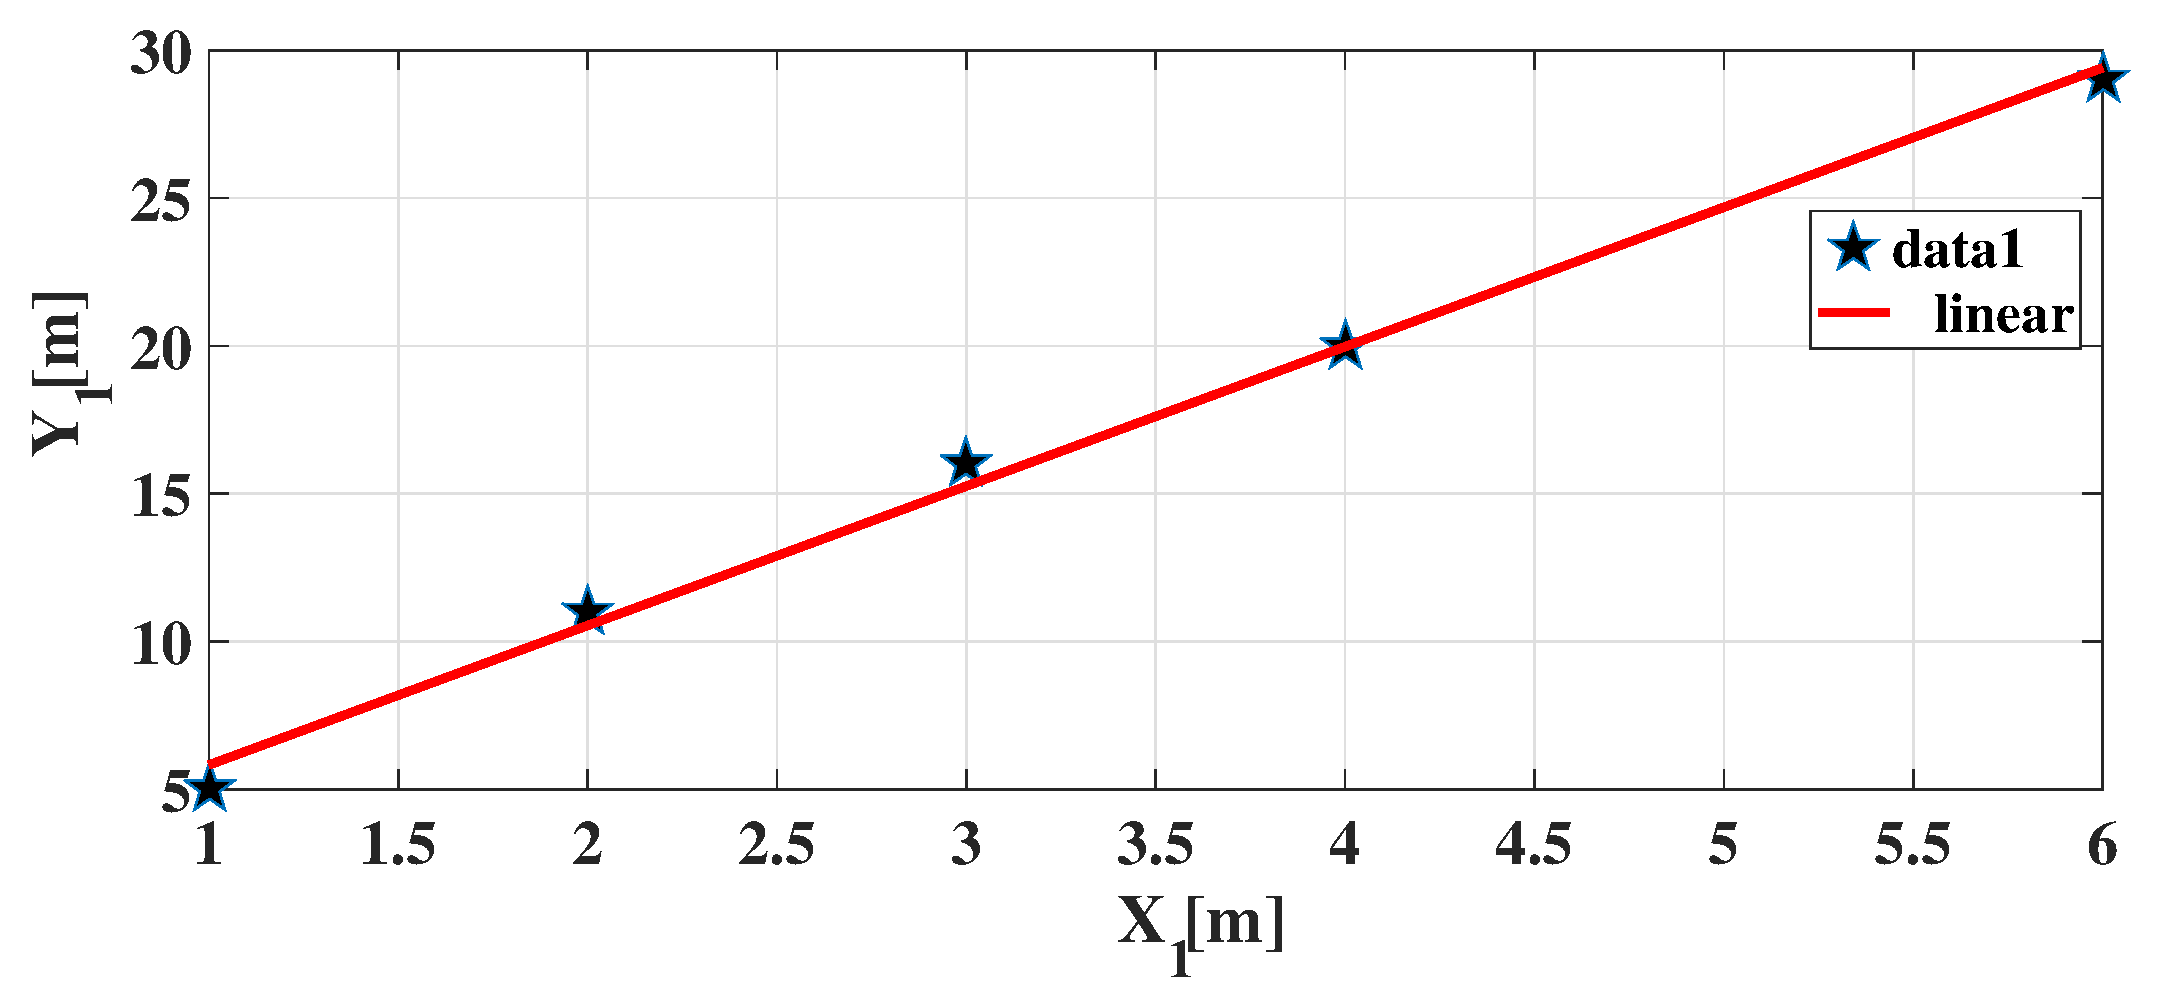
\includegraphics[scale=0.23]{fig} %[se define tamaño de la figura]{nombre del archivo con la figura}
\caption{Nombre descriptivo de la figura.} %Numera y titula la gráfica
\label{lvdt4} %Permite referenciar la grafica en el texto EJ: en la gráfica \ref{lvdt4} se observa...
\end{figure}

\subsection{Figuras en \LaTeX}
Para anexar una gráfica de datos se recomienda que sea en formato \textbf{eps} o \textbf{ps}, que puede generarse usando MATLAB como se muestra en \cite{imagenes}. También existen otras herramientas de generación de gráficos como Gnuplot \cite{GNUp}.

Se pueden modificar la posición y el tamaño de una figura, y anexar subfiguras. Si se desea anexar imágenes extraídas de otras fuentes (por ejemplo Internet), estas deben poseer buena resolución y preferiblemente estar en formato \textbf{png}.

Toda figura reportada en el documento debe tener referencia en el texto (por ejemplo: en la figura \ref{lvdt4} se presenta la característica $X_1$ contra $Y_1$).

Por otro lado, para crear esquemáticos de circuitos, diagramas de bloques y de flujo, pueden usarse herramientas como DIA \cite{dia} o XCircuit \cite{xcircuit}, u otros programas que permitan salvar preferiblemente gráficos en formatos \textbf{eps} o \textbf{ps}. En la figura \ref{diafig} se presenta un diagrama creado en XCircuit.
\begin{figure}[H] %[H] obliga a la figura a quedar en la misma posición en el texto final que en el archivo .tex, [t] coloca la figura en la parte superior de la página, [b] coloca la figura en la parte inferior de la página. 
\centering  %Centra la figura
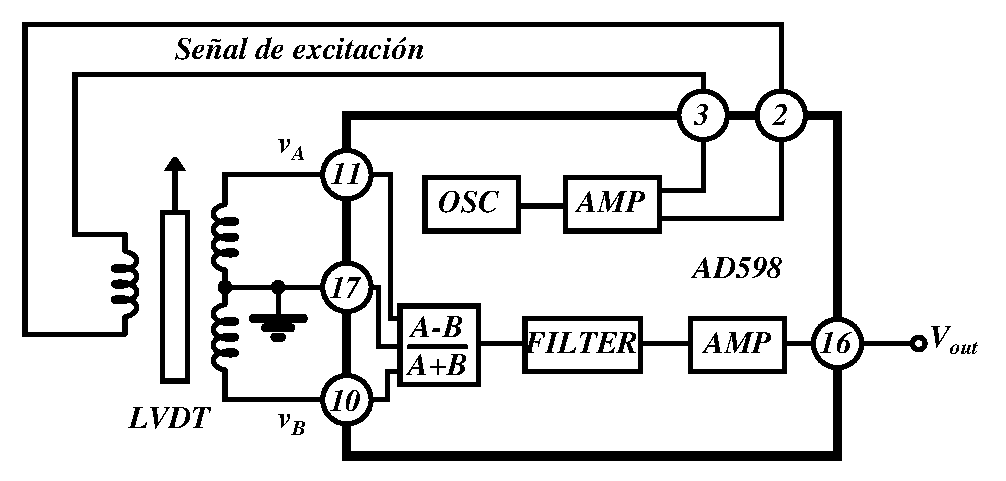
\includegraphics[scale=0.5]{LVDT4} %[se define tamaño de la figura]{nombre del archivo con la figura}
\caption{Diagrama del integrado AD598.} %Numera y da título a la gráfica
\label{diafig} %Permite referenciar la grafica en el texto EJ: en la gráfica \ref{lvdt4} se observa...
\end{figure}
%%%%%%%%%%%%%%%%%%%%%%%%%%%%%%%%%%%%%%

%%%%%%%%%%%%%%%%%%%%%%%%%%%%%%%
%%%%%%%%% ECUACIONES %%%%%%%%%%
%%%%%%%%%%%%%%%%%%%%%%%%%%%%%%%
\subsection{Ecuaciones en \LaTeX}

\begin{multline}\label{eqID}
\int^{r_2}_{0} F\left(r,\varphi\right)drd\varphi=\left[\sigma r_2/\left(2\mu_0\right)\right] \\ \cdot \int^{\infty}_{0} exp\left(-\lambda|z_j-z_i|\right)\lambda^{-1}J_1\left(\lambda r_2\right)J_0\left(\lambda r_i\right)d\lambda
%I_D=\frac{q N_A n_i^2}{N_D}\left(\frac{\alpha V_{GS}^2}{\mu_o}\right)^3
\end{multline}

Las ecuaciones se deben generar en \LaTeX (revisar el codigo fuente), no se deben anexar imágenes de ecuaciones. Por otro lado, para hacer referencia a una ecuación en el texto  se usa el mismo comando usado para la referencia de figuras y tablas pero dentro de paréntesis (por ejemplo: en (\ref{eqID}) se presenta la expresión para...).

Se pueden reportar procedimientos matemáticos sin enumerarlos como se muestra a continuación:
\begin{gather*}
i=\frac{v}{R}\Longrightarrow i=\frac{5}{500}=10 mA
\end{gather*}
%%%%%%%%%%%%%%%%%%%%%%%%%%%%%%%

%%%%%%%%%%%%%%%%%%%%%%%%%%%
%%%%%%%%% TABLAS %%%%%%%%%%
%%%%%%%%%%%%%%%%%%%%%%%%%%%
\subsection{Tablas en \LaTeX}
A continuación se presenta un ejemplo de tabla en \LaTeX (revisar el código fuente).

\begin{table}[H]
\makegapedcells
\centering
\caption{Nombre de la tabla}
\begin{tabular}{c l l}\hline\hline
\multirow{2}{*}{Symbol} & \multicolumn{1}{c}{\multirow{2}{*}{Quantity}} & \multicolumn{1}{c}{Conversion from Gaussian and}\\ 
& & \multicolumn{1}{c}{CGS EMU to SI}\\ \hline
$\Phi$ & magnetic flux & 1 Mx $\rightarrow$ 10$^{-8}$ Wb=10$^{-8}$ V.s \\
\multirow{2}{*}{$B$} & magnetic flux density, & \multirow{2}{*}{1 G $\rightarrow$ 10$^{-4}$ T = 10$^{-4}$ Wb/m$^2$}\\
& magnetic induction & \\
$H$ & magnetic field strength & 1 Oe $\rightarrow$ 10$^3$/(4$\pi$) A/m\\
\multirow{2}{*}{$m$} & \multirow{2}{*}{magnetic moment} & 1 erg/G=1 emu \\ 
& & $\rightarrow$ 10$^{-3}$ A.m$^2$=10$^{-3}$ J/T\\
\multirow{2}{*}{$M$} & \multirow{2}{*}{magnetization} & 1 erg/(G.cm$^3$)=1 emu/cm$^3$ \\ 
& & $\rightarrow$ 10$^3$ A/m\\ 
4$\pi M$& magnetization & 1 G $\rightarrow$ 10$^3$/(4$\pi$) A/m \\ 
$\sigma$ & specific magnetization & 1 erg/(G.g)=1 emu/g $\rightarrow$ 1 A.m$^2$/kg\\ 
$\chi$, $\kappa$ & susceptibility & 1 $\rightarrow$ 4$\pi$ \\ 
$N$, $D$ & demagnetizing factor & 1 $\rightarrow$ 1/(4$\pi$)\\ \hline\hline
\multicolumn{3}{p{8.5cm}}{Todo comentario o aclaración sobre la tabla va en este espacio. Toda tabla debe estar numerada y con su respectivo nombre.}\\
\end{tabular}
\label{table1}
\end{table}

Para hacer referencia a una tabla en el texto se usa el mismo comando que para las figuras y ecuaciones (por ejemplo: en la tabla \ref{table1} se muestran algunos ejemplos de variables asociadas al electromagnetismo).
%%%%%%%%%%%%%%%%%%%%%%%%%%%

%%%%%%%%%%%%%%%%%%%%%%%%%%%%%%
%%%%% CITAR BIBLIOGRAFIA %%%%%
%%%%%%%%%%%%%%%%%%%%%%%%%%%%%%
\subsection{Citar en formato IEEE en \LaTeX}
Para citar referencias bibliográficas se usa el comando \texttt{\char`\\ cite}. En \cite{nombre_para_citar} se muestran los campos que deben llenarse en una referencia, en \cite{kopka} se muestra un ejemplo, y en \cite{link} se muestra como citar un enlace. Preferiblemente citar libros y artículos.
%%%%%%%%%%%%%%%%%%%%%%%%%%%%%%

%%%%%%%%%%%%%%%%%%%%%%%%%%%%%%%%%%%%
%%% CUARTA SECCIÓN DEL DOCUMENTO %%%
%%%%%%%%%%%%%%%%%%%%%%%%%%%%%%%%%%%%
\section{Conclusiones}
Reportar en tercera persona las diferentes conclusiones producto de la práctica de laboratorio desarrollada. En las conclusiones se debe evidenciar la adquisición de las competencias a evaluar.
%%%%%%%%%%%%%%%%%%%%%%%%%%%%%%%%%%%%

\ifCLASSOPTIONcaptionsoff
  \newpage
\fi

%%%%%%%%%%%%%%%%%%%%%%%%%%
%%%%%% BIBLIOGRAFIA %%%%%%
%%%%%%%%%%%%%%%%%%%%%%%%%%
\begin{thebibliography}{1}

\bibitem{imagenes}
Youtube, canal schaparro. \url{https://youtu.be/IhvF6iY7n5k}. Recuperado el 30 de Enero de 2017.

\bibitem{GNUp}
Gnuplot homepage. \url{http://www.gnuplot.info/}. Recuperado el 26 de Julio de 2018.

\bibitem{dia}
Dia Diagram Editor. \url{https://sourceforge.net/projects/dia-installer/}. Recuperado el 30 de Enero de 2017.

\bibitem{xcircuit}
XCircuit, Open Circuit Design. \url{http://opencircuitdesign.com/xcircuit/}. Recuperado el 26 de Julio de 2018.

\bibitem{nombre_para_citar}
Inicial1.~Apellido1 and Inicial2.~Apellido2, \emph{Nombre de libro}, \#edición~ed.\hskip 1em plus
  0.5em minus 0.4em\relax Ciudad, País: Editorial, año.

\bibitem{kopka}
H.~Kopka and P.~W. Daly, \emph{A Guide to \LaTeX}, 3rd~ed.\hskip 1em plus
  0.5em minus 0.4em\relax Harlow, England: Addison-Wesley, 1999.

\bibitem{link}
Overleaf. \url{https://www.overleaf.com/}. Recuperado el 02 de Febrero de 2017.

\end{thebibliography}
%%%%%%%%%%%%%%%%%%%%%%%%%%

\end{document}
%%%%%%%%%%%%%%%%%%%%%%%%%%%%%%%%
%%%%%% FIN DEL DOCUMENTO %%%%%%%
%%%%%%%%%%%%%%%%%%%%%%%%%%%%%%%%




